\item If $\vec{v}$ is a non-zero vector of dimension $3\times 1$, then the matrix
$\vec{A} = \vec{v}\vec{v}^{\top}$ has a rank = \rule{1cm}{0.01pt} 
\hfill\brak{\text{IN 2017}}
\item \figref{fig:placeholder_1} shows a shape $ABC$ and its mirror image $A_1B_1C_1$ across the horizontal axis ($X$ axis). 
The coordinate transformation matrix that maps $ABC$ to $A_1B_1C_1$ is 

\hfill\brak{\text{IN 2017}}
\begin{figure}[H]
    \centering
    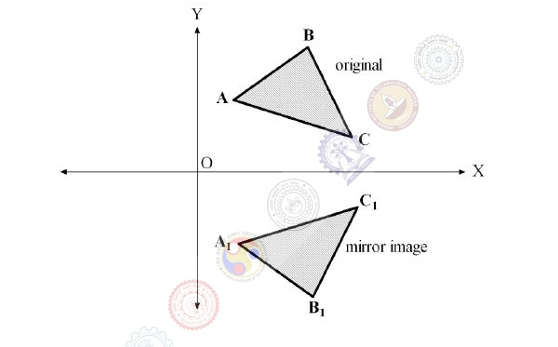
\includegraphics[width=0.5\columnwidth]{GATE/2017/IN/figs/Q-2.png}
    \caption{}
    \label{fig:placeholder_1}
\end{figure}
\begin{enumerate}
\begin{multicols}{4}
    \item $\myvec{0 & 1 \\ 1 & 0}$
    \item $\myvec{-1 & 0 \\ 1 & 0}$
    \item $\myvec{0 & 1 \\ -1 & 0}$
    \item $\myvec{0 & -1 \\ 1 & 0}$
\end{multicols}
\end{enumerate}
\item The eigenvalues of the matrix 
$\vec{A} = \myvec{1 & -1 & 5 \\ 0 & 5 & 6 \\ 0 & -6 & 5 }$
are  \hfill\brak{\text{IN 2017}}
\begin{enumerate}
\begin{multicols}{4}
    \item $-1, 5, 6$
    \item $1, -5 \pm j6$
    \item $1, 5 \pm j6$
    \item $1, 5, 5$    
\end{multicols}
\end{enumerate}
\item The connection of two $2$-port networks is shown in \figref{fig:placeholder_3}. The $ABCD$ parameters of $N_1$ and $N_2$ are 
$$\myvec{A & B \\ C & D}_{N1} = \myvec{1 & 5 \\ 0 & 1}$$ and $$\myvec{A & B \\ C & D}_{N2} = \myvec{0.2 & 1 \\ 1 & 1}$$
\begin{figure}[H]
    \centering
    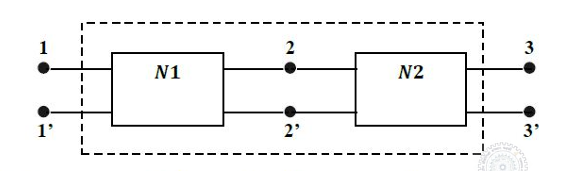
\includegraphics[width=0.5\columnwidth]{GATE/2017/IN/figs/Q-7.png}
    \caption{}
    \label{fig:placeholder_3}
\end{figure}
The $ABCD$ parameters of the combined 2-port network are \hfill\brak{\text{IN 2017}}
\begin{enumerate}
\begin{multicols}{4}
    \item $\myvec{2 & 5 \\ 0.2 & 1}$
    \item $\myvec{0.5 & 1 \\ -0.5 & 1}$
    \item $\myvec{0.5 & 5 \\ 2 & 1}$
    \item $\myvec{0.5 & 5 \\ 1 & 2}$
\end{multicols}
\end{enumerate}
\item A circuit consisting of dependent and independent sources is shown in \figref{fig:placeholder_4}. If the voltage at Node-1 is $-1$ V, then the voltage at Node-2 is \rule{1cm}{0.01pt}
\hfill\brak{\text{IN 2017}}
\begin{figure}[H]
    \centering
    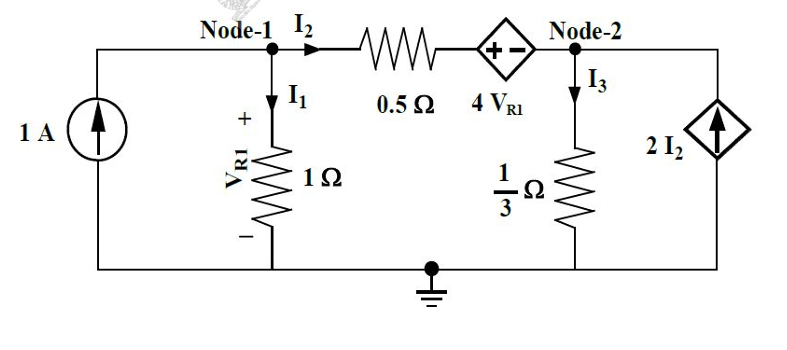
\includegraphics[width=0.6\columnwidth]{GATE/2017/IN/figs/Q-8.png}
    \caption{}
    \label{fig:placeholder_4}
\end{figure}
\item The angle between two vectors $\vec{x}_1 = \myvec{2& 6& 14}^{\top}$ and $\vec{x}_2 = \myvec{-12& 8& 16}^{\top}$ in radian is \rule{1cm}{0.01pt} 
\hfill\brak{\text{IN 2017}}
\item Consider two discrete-time signals   
$x_1\brak{n} = \cbrak{1, 1}$ and $x_2 \brak{n} = \{1, 2\}$ for $n = 0, 1$. 
The Z-transform of $x \brak{n} = x_1 \brak{n} * x_2 \brak{n}$ is \hfill\brak{\text{IN 2017}}
\begin{enumerate}
\begin{multicols}{4}
    \item $1 + 2z^{-1} + 3z^{-2}$
    \item $z^2 + 3z + 2$
    \item $1 + 3z^{-1} + 2z^{-2}$
    \item $z^{-2} + 3z^{-3} + 2z^{-4}$
\end{multicols}
\end{enumerate}

